\documentclass{standalone}
\usepackage{tikz}
\usetikzlibrary{patterns, positioning}
\usepackage[sfdefault]{ClearSans} %% option 'sfdefault' activates Clear Sans as the default text font
\usepackage[T1]{fontenc}

\begin{document}
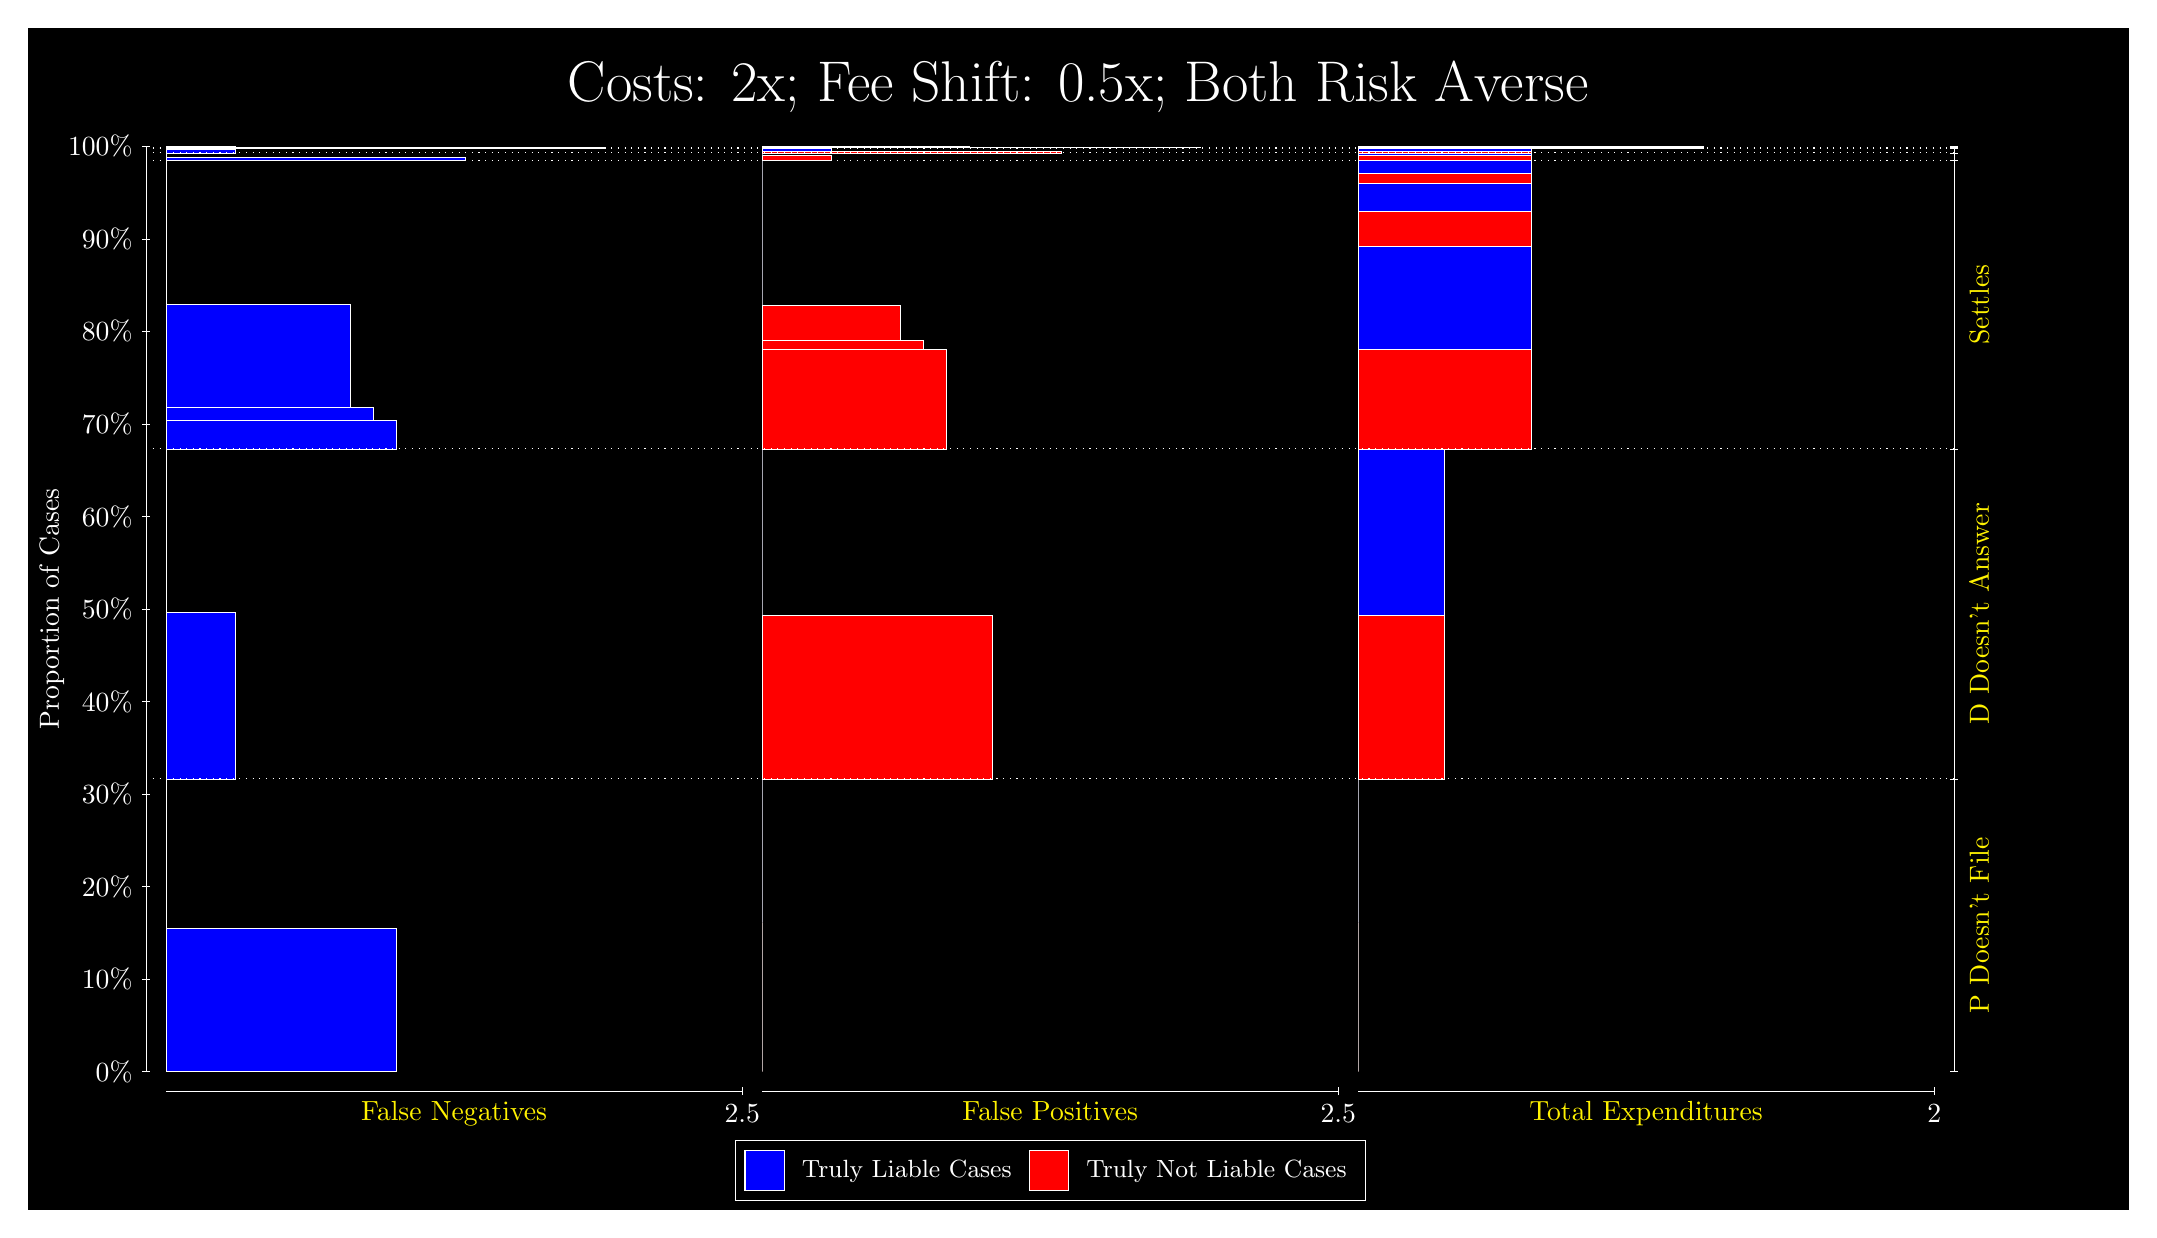
\begin{tikzpicture}
\draw[fill=black] (0,0) rectangle (26.667,15);
\draw[text=white] (0,13.5) rectangle (26.667,15) node[midway] {\huge Costs: 2x; Fee Shift: 0.5x; Both Risk Averse};
\draw[white, very thin] (1.5,1.75) -- (1.5,13.5);
\node[rotate=90, text=white, anchor=center] at (0.3, 7.625) {Proportion of Cases};
\draw[white, very thin] (1.45,1.75) -- (1.55,1.75);
\node[text=white, anchor=east] at (1.45, 1.75) {0\%};
\draw[white, very thin] (1.45,2.925) -- (1.55,2.925);
\node[text=white, anchor=east] at (1.45, 2.925) {10\%};
\draw[white, very thin] (1.45,4.1) -- (1.55,4.1);
\node[text=white, anchor=east] at (1.45, 4.1) {20\%};
\draw[white, very thin] (1.45,5.275) -- (1.55,5.275);
\node[text=white, anchor=east] at (1.45, 5.275) {30\%};
\draw[white, very thin] (1.45,6.45) -- (1.55,6.45);
\node[text=white, anchor=east] at (1.45, 6.45) {40\%};
\draw[white, very thin] (1.45,7.625) -- (1.55,7.625);
\node[text=white, anchor=east] at (1.45, 7.625) {50\%};
\draw[white, very thin] (1.45,8.8) -- (1.55,8.8);
\node[text=white, anchor=east] at (1.45, 8.8) {60\%};
\draw[white, very thin] (1.45,9.975) -- (1.55,9.975);
\node[text=white, anchor=east] at (1.45, 9.975) {70\%};
\draw[white, very thin] (1.45,11.15) -- (1.55,11.15);
\node[text=white, anchor=east] at (1.45, 11.15) {80\%};
\draw[white, very thin] (1.45,12.325) -- (1.55,12.325);
\node[text=white, anchor=east] at (1.45, 12.325) {90\%};
\draw[white, very thin] (1.45,13.5) -- (1.55,13.5);
\node[text=white, anchor=east] at (1.45, 13.5) {100\%};

\draw[white, very thin] (24.457,1.75) -- (24.457,13.5);
\draw[white, very thin] (24.407,1.75) -- (24.507,1.75);
\node[anchor=west] at (24.407, 1.75) {};
\draw[white, very thin] (24.407,5.4674) -- (24.507,5.4674);
\node[anchor=west] at (24.407, 5.4674) {};
\draw[white, very thin] (24.407,9.6588) -- (24.507,9.6588);
\node[anchor=west] at (24.407, 9.6588) {};
\draw[white, very thin] (24.407,13.322) -- (24.507,13.322);
\node[anchor=west] at (24.407, 13.322) {};
\draw[white, very thin] (24.407,13.416) -- (24.507,13.416);
\node[anchor=west] at (24.407, 13.416) {};
\draw[white, very thin] (24.407,13.478) -- (24.507,13.478);
\node[anchor=west] at (24.407, 13.478) {};
\draw[white, very thin] (24.407,13.489) -- (24.507,13.489);
\node[anchor=west] at (24.407, 13.489) {};
\draw[white, very thin] (24.407,13.5) -- (24.507,13.5);
\node[anchor=west] at (24.407, 13.5) {};

\draw[white, very thin, fill=blue] (1.75,1.75) rectangle (4.6775,3.5746);
\draw[white, very thin, fill=red] (1.75,3.5746) rectangle (1.75,5.4674);
\draw[white, very thin, fill=blue] (1.75,5.4674) rectangle (2.6283,7.5848);
\draw[white, very thin, fill=red] (1.75,7.5848) rectangle (1.75,9.6588);
\draw[white, very thin, fill=blue] (1.75,9.6588) rectangle (4.6775,10.022);
\draw[white, very thin, fill=blue] (1.75,10.022) rectangle (4.3848,10.187);
\draw[white, very thin, fill=blue] (1.75,10.187) rectangle (4.092,11.499);
\draw[white, very thin, fill=red] (1.75,11.499) rectangle (1.75,13.322);
\draw[white, very thin, fill=blue] (1.75,13.322) rectangle (5.5558,13.358);
\draw[white, very thin, fill=red] (1.75,13.358) rectangle (1.75,13.416);
\draw[white, very thin, fill=blue] (1.75,13.416) rectangle (2.6283,13.461);
\draw[white, very thin, fill=red] (1.75,13.461) rectangle (1.75,13.478);
\draw[white, very thin, fill=blue] (1.75,13.478) rectangle (7.3123,13.483);
\draw[white, very thin, fill=red] (1.75,13.483) rectangle (1.75,13.489);
\draw[white, very thin, fill=blue] (1.75,13.489) rectangle (2.6283,13.496);
\draw[white, very thin, fill=red] (1.75,13.496) rectangle (1.75,13.5);
\draw[white, very thin, fill=red] (9.3189,1.75) rectangle (9.3189,3.6428);
\draw[white, very thin, fill=blue] (9.3189,3.6428) rectangle (9.3189,5.4674);
\draw[white, very thin, fill=red] (9.3189,5.4674) rectangle (12.246,7.5414);
\draw[white, very thin, fill=blue] (9.3189,7.5414) rectangle (9.3189,9.6588);
\draw[white, very thin, fill=red] (9.3189,9.6588) rectangle (11.661,10.917);
\draw[white, very thin, fill=red] (9.3189,10.917) rectangle (11.368,11.037);
\draw[white, very thin, fill=red] (9.3189,11.037) rectangle (11.075,11.482);
\draw[white, very thin, fill=blue] (9.3189,11.482) rectangle (9.3189,13.322);
\draw[white, very thin, fill=red] (9.3189,13.322) rectangle (10.197,13.38);
\draw[white, very thin, fill=blue] (9.3189,13.38) rectangle (9.3189,13.416);
\draw[white, very thin, fill=red] (9.3189,13.416) rectangle (13.125,13.433);
\draw[white, very thin, fill=blue] (9.3189,13.433) rectangle (10.197,13.478);
\draw[white, very thin, fill=red] (9.3189,13.478) rectangle (10.197,13.484);
\draw[white, very thin, fill=blue] (9.3189,13.484) rectangle (9.3189,13.489);
\draw[white, very thin, fill=red] (9.3189,13.489) rectangle (14.881,13.492);
\draw[white, very thin, fill=blue] (9.3189,13.492) rectangle (11.954,13.5);
\draw[white, very thin, fill=red] (16.888,1.75) rectangle (16.888,3.6428);
\draw[white, very thin, fill=blue] (16.888,3.6428) rectangle (16.888,5.4674);
\draw[white, very thin, fill=red] (16.888,5.4674) rectangle (17.986,7.5414);
\draw[white, very thin, fill=blue] (16.888,7.5414) rectangle (17.986,9.6588);
\draw[white, very thin, fill=red] (16.888,9.6588) rectangle (19.083,10.917);
\draw[white, very thin, fill=blue] (16.888,10.917) rectangle (19.083,12.229);
\draw[white, very thin, fill=red] (16.888,12.229) rectangle (19.083,12.674);
\draw[white, very thin, fill=blue] (16.888,12.674) rectangle (19.083,13.037);
\draw[white, very thin, fill=red] (16.888,13.037) rectangle (19.083,13.157);
\draw[white, very thin, fill=blue] (16.888,13.157) rectangle (19.083,13.322);
\draw[white, very thin, fill=red] (16.888,13.322) rectangle (19.083,13.38);
\draw[white, very thin, fill=blue] (16.888,13.38) rectangle (19.083,13.416);
\draw[white, very thin, fill=red] (16.888,13.416) rectangle (19.083,13.433);
\draw[white, very thin, fill=blue] (16.888,13.433) rectangle (19.083,13.478);
\draw[white, very thin, fill=red] (16.888,13.478) rectangle (21.279,13.484);
\draw[white, very thin, fill=blue] (16.888,13.484) rectangle (21.279,13.489);
\draw[white, very thin, fill=red] (16.888,13.489) rectangle (21.279,13.492);
\draw[white, very thin, fill=blue] (16.888,13.492) rectangle (21.279,13.5);
\draw[white, dotted] (1.5,5.4674) -- (24.457,5.4674);
\draw[white, dotted] (1.5,9.6588) -- (24.457,9.6588);
\draw[white, dotted] (1.5,13.322) -- (24.457,13.322);
\draw[white, dotted] (1.5,13.416) -- (24.457,13.416);
\draw[white, dotted] (1.5,13.478) -- (24.457,13.478);
\draw[white, dotted] (1.5,13.489) -- (24.457,13.489);
\draw[white, very thin] (1.75,1.5) -- (9.0689,1.5);
\node[text=yellow, anchor=north] at (5.4094, 1.5) {False Negatives};
\draw[white, very thin] (9.0689,1.45) -- (9.0689,1.55);
\node[text=white, anchor=north] at (9.0689, 1.45) {2.5};

\draw[white, very thin] (9.3189,1.5) -- (16.638,1.5);
\node[text=yellow, anchor=north] at (12.978, 1.5) {False Positives};
\draw[white, very thin] (16.638,1.45) -- (16.638,1.55);
\node[text=white, anchor=north] at (16.638, 1.45) {2.5};

\draw[white, very thin] (16.888,1.5) -- (24.207,1.5);
\node[text=yellow, anchor=north] at (20.547, 1.5) {Total Expenditures};
\draw[white, very thin] (24.207,1.45) -- (24.207,1.55);
\node[text=white, anchor=north] at (24.207, 1.45) {2};

\node[text=yellow, centered, rotate=90] at (24.777, 3.6087) {P Doesn't File};
\node[text=yellow, centered, rotate=90] at (24.777, 7.5631) {D Doesn't Answer};
\node[text=yellow, centered, rotate=90] at (24.777, 11.49) {Settles};





\draw (12.978300999999998,1.5) node[draw=none] (baseCoordinate) {};
\begin{scope}[align=center]
        \matrix[scale=0.5, draw=white, below=0.5cm of baseCoordinate, nodes={draw}, column sep=0.1cm]{
            \node[rectangle, draw, minimum width=0.5cm, minimum height=0.5cm, fill=blue] {}; &
            \node[draw=none, font=\small, text=white] (B) {Truly Liable Cases}; &
            \node[rectangle, draw, minimum width=0.5cm, minimum height=0.5cm, fill=red] {}; &
            \node[draw=none, font=\small, text=white] (B) {Truly Not Liable Cases}; \\
            };
\end{scope}

\end{tikzpicture}
\end{document}